\documentclass[conference]{IEEEtran}
\IEEEoverridecommandlockouts
% The preceding line is only needed to identify funding in the first footnote. If that is unneeded, please comment it out.
\usepackage{cite}
\usepackage{amsmath,amssymb,amsfonts}
%\usepackage{algorithmic}
\usepackage{algorithm}
\usepackage{algpseudocode} % 更好控制语法结构
\usepackage{graphicx}
\usepackage{textcomp}
\usepackage{xcolor}
\usepackage{tabularx}
\usepackage{epstopdf}
\usepackage{pifont}
\usepackage{makecell}
\usepackage{hyperref}
\hypersetup{
   hypertex=true,
   colorlinks=true,
   linkcolor=blue,
   anchorcolor=blue,
   citecolor=blue
}
\def\BibTeX{{\rm B\kern-.05em{\sc i\kern-.025em b}\kern-.08em
    T\kern-.1667em\lower.7ex\hbox{E}\kern-.125emX}}
\begin{document}

\title{Mode-Adaptive Control of DC--DC Converters via Action-Regularized PPO-Based Reinforcement Learning\\}

\author{
    \IEEEauthorblockN{Chuanchuan Liang, Chaohong Zhang, Xueyong Zhang, and Weifeng Sun}
    \IEEEauthorblockA{
        Department of Integrated Circuits, Southeast University\\Nanjing 210096, China\\
        Email: \{230240065, 230258719, xueyong.zhang, swffrog\}@seu.edu.cn
    }
}

% \author{\IEEEauthorblockN{Chuanchuan Liang}
% \IEEEauthorblockA{\textit{Department of Integrated Circuits} \\
% \textit{Southeast University}\\
% Nanjing, Jiangsu, China \\
% 230240065@seu.edu.cn}

% \and
% \IEEEauthorblockN{Xueyong Zhang}
% \IEEEauthorblockA{\textit{Department of Integrated Circuits} \\
% \textit{Southeast University}\\
% Nanjing, Jiangsu, China \\
% xueyong.zhang@seu.edu.cn}
% \and
% \IEEEauthorblockN{Weifeng Sun}
% \IEEEauthorblockA{\textit{Department of Integrated Circuits} \\
% \textit{Southeast University}\\
% Nanjing, Jiangsu, China \\
% swffrog@seu.edu.cn}}

\maketitle

\begin{abstract}
DC--DC converters are critical components in modern power electronic systems. However, their performance can be significantly affected by nonlinear dynamics, parameter uncertainties, and mode transitions, especially under constant power loads that introduce negative impedance characteristics. To address these challenges, this work proposes a model-free control strategy based on the Proximal Policy Optimization (PPO) algorithm within a deep reinforcement learning (DRL) framework. The proposed controller incorporates four core innovations: 
(i) an expanded observation space including inductor current to improve adaptability and transient response;  
(ii) a reward function designed using the square root of normalized voltage error to enhance steady-state precision and convergence speed;  
(iii) an action regularization mechanism that discourages abrupt duty cycle changes, promoting smooth switching and reducing stress on components; and  
(iv) a unified PPO policy capable of seamless operation across continuous and discontinuous conduction modes without explicit mode detection.
The controller is trained using a high-fidelity MATLAB/Simulink simulation environment and is evaluated under a wide range of operating conditions, including input voltage variation, load disturbances, and component uncertainties. Simulation results confirm significant improvements in voltage regulation accuracy, dynamic performance, and robustness.
\end{abstract}


\begin{IEEEkeywords}
DC–DC converters, deep reinforcement learning, Proximal Policy Optimization, mode transition, action regularization
\end{IEEEkeywords}

\section{Introduction}

DC--DC converters play a vital role in power electronic systems by enabling efficient voltage regulation across a broad range of applications, such as electric vehicles, aerospace systems, and renewable energy platforms. However, their performance is often degraded by nonlinear dynamics, parametric uncertainties, conduction mode transitions, and external disturbances. These effects are particularly pronounced under constant power load conditions, which introduce negative impedance characteristics and thus tend to destabilize the converter system.

Traditional control strategies, such as proportional--integral--derivative (PID) control, sliding mode control, and model predictive control, typically rely on accurate system models and linear approximations. These assumptions limit controller robustness when applied to high-frequency switching systems and time-varying load conditions~\cite{cui2021voltage}. Model-free approaches using neural networks and fuzzy logic have been investigated as alternatives, yet they often exhibit limited generalization and poor adaptability to unmodeled dynamics \cite{zhao2020overview,benachour2024generalized}.

Recent developments in deep reinforcement learning (DRL) have shown promising results in controlling complex nonlinear systems without explicit modeling~\cite{gheisarnejad2020iot,feng2024deep}. Algorithms such as Deep Deterministic Policy Gradient (DDPG), Twin Delayed DDPG (TD3), and Deep Q-Network (DQN) have been explored for their application in converter control~\cite{cui2021voltage,tang2021artificial,ye2024td3,muktiadji2024twin,cui2021transferring,kishore2022performance}. However, major challenges remain—particularly in the robust handling of conduction mode transitions, the design of observation spaces capable of capturing system dynamics, and the assurance of control smoothness under dynamic operating conditions~\cite{min2022voltage,ye2024deep}.

To address these limitations, this paper presents a Proximal Policy Optimization (PPO)-based DRL controller with four distinctive features:  
(i) an observation space augmented with inductor current dynamics for enhanced transient adaptability;  
(ii) a reward function constructed using the square root of normalized voltage error to improve convergence near steady-state;  
(iii) a control smoothness regularization term that penalizes rapid duty cycle variations to improve switching stability; and  
(iv) a unified PPO policy that operates consistently across conduction modes without the need for explicit mode detection or switching logic.


%The proposed controller is trained and tested on a high-fidelity switching model of the converter. Extensive simulation results demonstrate improved voltage regulation, enhanced dynamic response, and superior robustness against parameter uncertainties, in comparison to traditional PI-based controllers~\cite{pi_vs_drl}.


\section{SYSTEM MODEL AND REINFORCEMENT LEARNING CONCEPT}

This section comprises two subsections. The first introduces the Buck converter model utilized for controller training and evaluation. The second presents the rationale for adopting the PPO algorithm, along with its mathematical formulation and structural benefits for power electronic control.

\subsection{System Model}

Fig.~\ref{fig:buck_model}(a) shows an ideal Buck converter, while Fig.~\ref{fig:buck_model}(b) presents a non-ideal variant including parasitic elements such as inductor resistance $R_L$, equivalent series resistance $R_C$ of the output capacitor, switch on-resistance $R_{\text{on}}$, and diode voltage drop $V_D$. The converter alternates between ON and OFF states per switching cycle [Figs.~\ref{fig:buck_model}(c) and (d)], forming a hybrid nonlinear system. A high-fidelity switching model is constructed to capture the fast time-scale dynamics critical to accurately representing converter behavior. This model serves as the simulation environment for training the DRL controller, enabling policy optimization under realistic electrical conditions.

%In this study, the converter is modeled in MATLAB/Simulink using a detailed switching model. The PPO agent interacts with the environment through a duty-cycle signal that is translated into a PWM signal to control the switching transistor. The environment returns observable states, including output voltage and inductor current, at each control step. This closed-loop interaction forms the training setup for the model-free control policy.




%\subsection{Conventional Control Method}

%To provide a performance benchmark, a conventional double-loop PI control strategy is implemented for the Buck converter. This method is widely adopted in industrial applications due to its simplicity and reasonable performance under nominal operating conditions.

%The control architecture consists of an outer voltage loop and an inner current loop. The outer voltage loop compares the measured output voltage $V_o(t)$ with the reference voltage $V_{\text{ref}}$ to generate a reference current $i_{\text{ref}}(t)$. The inner loop then compares $i_{\text{ref}}(t)$ with the actual inductor current $i_L(t)$ to generate the duty cycle $d(t)$, which is applied to the PWM generator.

%The control laws for the two loops are expressed as:

%\begin{equation}
%\begin{aligned}
%i_{\text{ref}}(t) &= K_{pv}(V_{\text{ref}} - V_o(t)) + K_{iv} \int_0^t (V_{\text{ref}} - V_o(\tau))\,d\tau \\
%d(t) &= K_{pi}(i_{\text{ref}}(t) - i_L(t)) + K_{ii} \int_0^t (i_{\text{ref}}(\tau) - i_L(\tau))\,d\tau
%\end{aligned}
%\end{equation}

%where $K_{pv}$ and $K_{iv}$ are the proportional and integral gains for the voltage loop, and $K_{pi}$ and $K_{ii}$ are the corresponding gains for the current loop.

%hile the double-loop PI controller achieves satisfactory performance under steady-state conditions, its effectiveness degrades in the presence of parameter perturbations or conduction mode transitions. Specifically, fixed-gain PI controllers are not inherently robust to variations in inductance, capacitance, or load resistance, and may require manual retuning. Furthermore, abrupt changes in control signals can induce overshoot, oscillations, or increased switching losses, which limits their applicability in scenarios with high dynamic uncertainty.

%This motivates the adoption of a model-free control approach capable of adapting to nonlinear dynamics and operating uncertainties without explicit system modeling or manual parameter tuning.
%The block diagram of conventional double-loop PI is shown in Fig. 2.

\subsection{Deep Reinforcement Learning}

DRL enables model-free control through agent-environment interaction guided by scalar rewards. In power electronic systems, DRL addresses nonlinearities, discontinuities, and unmodeled disturbances without requiring explicit plant models. For converter applications, the RL algorithm should support: (i) continuous action spaces, (ii) model-free operation, (iii) hyperparameter robustness, and (iv) high sample efficiency~\cite{mazaheri2024deep}. As summarized in Table~\ref{tab:DRLcompare}, PPO satisfies these criteria and ensures stable convergence via conservative policy updates.

\begin{figure}[!t]
  \centering
  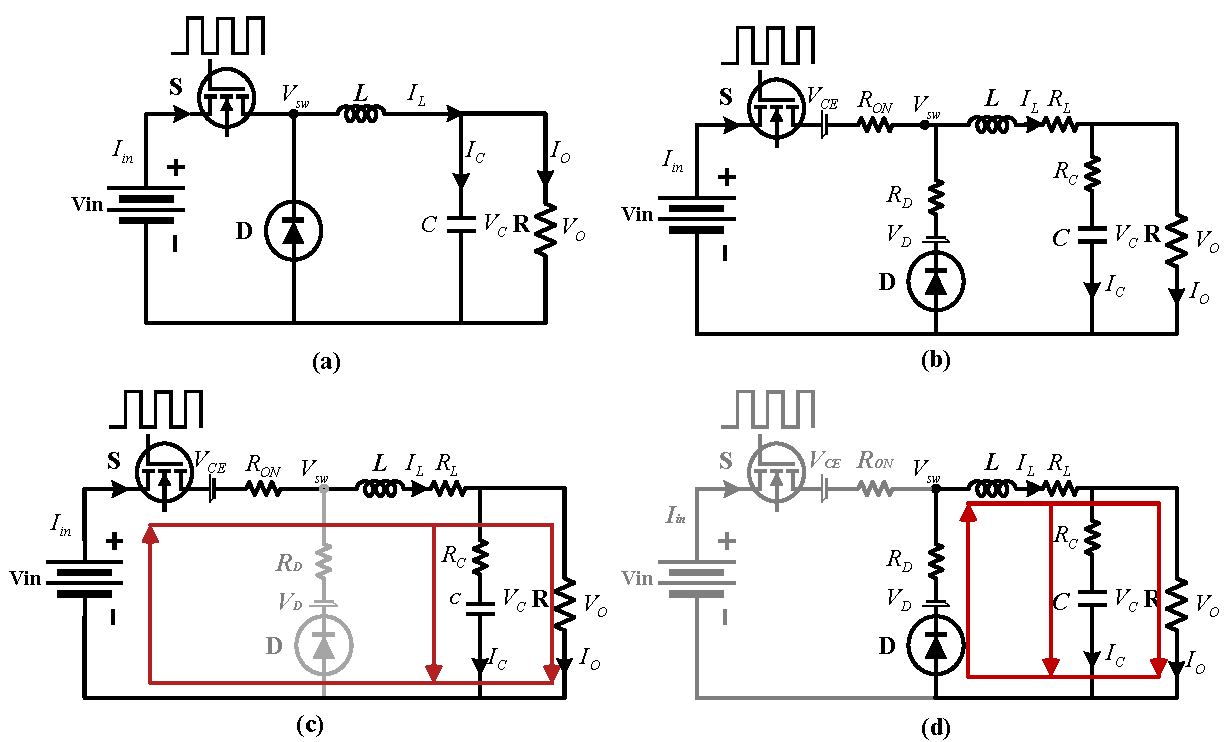
\includegraphics[width=0.48\textwidth]{figs/buck_model4.pdf}
  \caption{(a) Ideal Buck converter; (b) Non-ideal converter with parasitic components; (c) ON-state equivalent circuit; (d) OFF-state equivalent circuit.}
  \label{fig:buck_model}
\end{figure}

\begin{figure}[t]
  \centering
  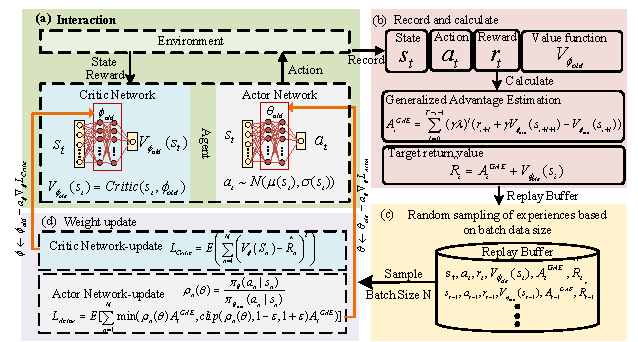
\includegraphics[width=0.48\textwidth]{figs/ppo_structure3.pdf}
  \caption{Architecture of the PPO-based model-free control framework.}
  \label{fig:PPO}
\end{figure}
% 替代对勾符号
\newcommand{\cmark}{\ding{51}} % 对勾
\newcommand{\xmark}{\ding{55}} % 叉号

% \begin{table*}[t]
% \centering
% \caption{Comparison of DRL algorithms for converter control.}
% \label{tab:DRLcompare}
% \begin{tabular}{lccccc}
% \hline\hline
% \textbf{Algorithm Type} & 
% \makecell[c]{\textbf{No Model} \\ \textbf{Required}} & 
% \makecell[c]{\textbf{Sample \&} \\ \textbf{Computation Efficient}} & 
% \makecell[c]{\textbf{Hyperparameter} \\ \textbf{Robustness}} & 
% \makecell[c]{\textbf{Continuous} \\ \textbf{Action Support}} \\
% \hline
% \textbf{Model-Free} &  &   &   &   \\
% Value-Based (e.g., DQN)       & \cmark & \cmark & \cmark & \xmark \\
% Policy-Based (e.g., PG)       & \cmark & \xmark & \xmark & \cmark \\
% Actor–Critic (e.g., PPO) & \cmark & \cmark\cmark\cmark & \cmark\cmark\cmark & \cmark \\
% Actor–Critic (e.g., TD3) & \cmark & \cmark\cmark & \cmark\cmark & \cmark \\
% Actor–Critic (e.g., DDPG) & \cmark & \cmark & \cmark & \cmark \\
% \hline
% \textbf{Model-Based}                               & \xmark & \cmark\cmark & \cmark\cmark & \cmark \\
% \hline
% \end{tabular}
% \end{table*}
\begin{table*}[t]
\centering
\caption{Comparison of representative DRL algorithms for DC--DC converter control.}
\label{tab:DRLcompare}
\begin{tabular}{lcccc}
\hline\hline
\textbf{Algorithm} & 
\textbf{Sample \& Computation Efficiency} & 
\textbf{Hyperparameter Robustness} & 
\textbf{Continuous Action Support} & 
\textbf{Model Requirement} \\
\hline
\textbf{Model-Free} &  &   &   &   \\
Value-Based (e.g., DQN)         & High     & High     & No      & No \\
Policy-Based (e.g., PG)         & Low      & Low      & Yes     & No \\
Actor--Critic (e.g., PPO)       & High & High & Yes     & No \\
Actor--Critic (e.g., TD3)       & Good     & Good     & Yes     & No \\
Actor--Critic (e.g., DDPG)      & Fair     & Fair     & Yes     & No \\
\hline
\textbf{Model-Based}     & Good     & Good     & Yes     & Yes \\
\hline
\end{tabular}

\end{table*}


%Traditional value-based methods such as Q-learning and DQN are restricted to discrete action spaces, making them unsuitable for high-resolution PWM control. While DDPG addresses this limitation through deterministic policies and supports continuous control, it suffers from instability during training due to Q-value overestimation. TD3 improves upon DDPG by using twin critics and delayed policy updates, enhancing convergence stability. However, TD3 can still be sensitive to hyperparameter settings and may require extensive tuning.

%Compared to these alternatives, PPO strikes a favorable balance between stability and performance. As an actor–critic algorithm, PPO combines the benefits of both policy-based and value-based approaches. It performs stable policy updates through a clipped surrogate objective, which constrains large policy deviations and reduces training oscillations. PPO also supports continuous action spaces and has been shown to offer strong robustness across various control scenarios.

The core contribution of PPO lies in its clipped surrogate objective, which constrains the policy update at each step to avoid excessively large deviations from the previous policy. The objective function is defined as:

\begin{equation}
L^{\text{CLIP}}(\theta) = \mathbb{E}_t \left[ \min \left( r_t(\theta) \hat{A}_t, \ \text{clip}(r_t(\theta), 1 - \epsilon, 1 + \epsilon) \hat{A}_t \right) \right]
\label{eq:ppo_clip}
\end{equation}

where $r_t(\theta) = \frac{\pi_\theta(a_t | s_t)}{\pi_{\theta_{\text{old}}}(a_t | s_t)}$ is the probability ratio between the current and previous policies, and $\hat{A}_t$ denotes the advantage estimate. The clipping threshold $\epsilon$ (typically 0.1–0.3) limits policy deviation to stabilize learning.

The PPO-clipped algorithm adopts an actor--critic framework, where the policy network maps system states to continuous control actions and the value network estimates expected returns, as shown in Algorithm~\ref{alg:ppo} and Fig.~\ref{fig:PPO}. The clipped surrogate objective constrains policy updates and prevents instability from abrupt changes, which is critical for fast-switching converters. By balancing conservatism and learning efficiency, PPO ensures stable training under nonlinear, noisy conditions and is well-suited for high-frequency converter control with stringent regulation requirements.





\begin{algorithm}[!t]
\caption{PPO-clipped}
\label{alg:ppo}
\begin{algorithmic}[1]
\State \textbf{Input:} Initial policy parameters $\theta_0$, initial value function parameters $\phi_0$
\For{$k = 0, 1, 2, \ldots$}
    \State Collect the set of trajectories $D_k = \{\tau_i\}$ by running the policy $\pi_k = \pi(\theta_k)$ in the environment.
    \State Compute rewards-to-go, $\hat{r}_t$, representing the cumulative sum of future rewards from time step $t$ onward.
    \State Compute advantage estimates, $\hat{A}_t$, based on the current value function $V_{\phi_k}$ which represents the expected return from a given state.
    \State Update the policy by maximizing the PPO-clip:
    \[
        \theta_{k+1} \leftarrow \arg\max_\theta L^{\text{CLIP}}(\theta)
    \]
   \State Fit the value function by regression with MSE:
    \[
        \phi_{k+1} \leftarrow \arg\min_\phi \frac{1}{|D_k||T|} \sum_{\tau \in D_k} \sum_{t=0}^{T} \left( V_\phi(s_t) - \hat{r}_t \right)^2
   \]
\EndFor
\end{algorithmic}
\end{algorithm}


\section{PROPOSED MODEL-FREE CONTROL}

The DRL control framework comprises an agent and an environment. The PPO agent interacts with the converter by observing system states, generating control actions, and receiving scalar rewards to guide policy optimization. The observation, action, and reward structures are described in the following subsections.


\subsection{Observation Space}

The observation vector consists of five key signals: input voltage $v_{\text{in}}$, inductor current $i_L$, output current $i_{\text{out}}$, reference voltage $v_{\text{ref}}$, and voltage error $e = v_{\text{ref}} - v_{\text{out}}$. To incorporate temporal information and better capture dynamic behavior, each signal is sampled at the current and previous time steps, resulting in a 10-dimensional observation vector.


\begin{equation}
\mathbf{obs}(t) =
\begin{bmatrix}
v_{\text{in}}(t),\ i_L(t),\ i_{\text{out}}(t),\ v_{\text{ref}}(t),\ e(t) \\
v_{\text{in}}(t{-}1),\ i_L(t{-}1),\ i_{\text{out}}(t{-}1),\ v_{\text{ref}}(t{-}1),\ e(t{-}1)
\end{bmatrix}
\label{eq:obs_vector}
\end{equation}

This formulation implicitly encodes temporal information, enabling the agent to infer system dynamics without reliance on explicit physical models.

\subsection{Action Space}
In contrast to discrete-action DRL controllers, the proposed PPO agent generates continuous-valued duty cycles, enabling high-resolution Pulse Width Modulation control. This design enhances transient performance and reduces steady-state error under dynamic operating conditions.


\subsection{Reward Function}
The reward function is formulated to jointly promote voltage tracking accuracy and smooth control behavior:

\begin{equation}
R_t =
\begin{cases}
-k_1 \sqrt{\left| e_{\text{norm}} \right|} - k_2 \left| e_{\text{action}} \right|, & \text{if } \left| e_{\text{norm}} \right| < 0.01 \\[6pt]
-k_3 \sqrt{\left| e_{\text{norm}} \right|}, & \text{otherwise}
\end{cases}
\label{eq:reward}
\end{equation}

where $e_{\text{norm}} = \frac{e_t}{V_{\text{ref}}}$ represents the normalized voltage error, and $e_{\text{action}} = a_t - a_{t-1}$ denotes the duty cycle variation. This structure penalizes both steady-state deviations and abrupt control changes, thereby encouraging precise regulation with smooth switching transitions.


\section{RESULTS AND DISCUSSION}

The PPO controller was trained in MATLAB/Simulink using the parameters listed in Tables~\ref{tab:buck_params} and~\ref{tab:trainparams}. As shown in Fig.~\ref{fig:training_curve}, the cumulative reward increased steadily over 300 episodes, indicating stable convergence and effective policy learning.

Robustness was evaluated under parameter perturbations limited to inductance and capacitance, each varied by $\pm30\%$ from their nominal values. As shown in Fig.~\ref{fig:indcap}, deviations in inductance (nominal: $0.47\,\mu\text{H}$) resulted in output voltage errors ranging from $-0.62\%$ to $+0.13\%$, while capacitance variations (nominal: $44\,\mu\text{F}$) produced errors between $-0.19\%$ and $-0.01\%$. These results demonstrate strong controller resilience and high steady-state voltage regulation accuracy under component uncertainties.

Dynamic performance was further evaluated under abrupt variations in input voltage, load current, and reference voltage, as shown in Fig.~\ref{fig:ccm_dcm}. These transients induced conduction mode transitions between continuous conduction mode (CCM) and discontinuous conduction mode (DCM), thereby testing the policy’s generalization capability beyond the training domain (indicated by red dashed lines). Across all test scenarios, the controller maintained stable operation without oscillations. The output voltage accurately tracked the reference, with steady-state errors constrained within $\pm0.7\%$. As shown in the transient insets of Fig.~\ref{fig:ccm_dcm}, both overshoot and undershoot were approximately $5\%$, and the system returned to steady-state within $10\,\mu\text{s}$ following each disturbance.



\begin{table}[t]
\caption{Buck Converter Parameters}
\label{tab:buck_params}
\centering
\begin{tabularx}{\linewidth}{>{\centering\arraybackslash}X >{\centering\arraybackslash}X >{\centering\arraybackslash}X}
\hline\hline
\textbf{Parameter} & \textbf{Symbol} & \textbf{Value} \\
\hline
Input voltage        & $V_{\text{in}}$         & $2 < V_{\text{in}} < 8$ V \\
Reference voltage    & $V_{\text{ref}}$        & $1.5 < V_{\text{in}} < 5$ V \\
Inductance           & $L$                    & 0.47 uH         \\
Capacitance          & $C$                    & 44 uF       \\
Inductor DCR         & $R_{\text{L}}$       & 3.7 $m\Omega$  \\
Capacitor ESR        & $R_{\text{C}}$       & 3 $m\Omega$ \\
Switching frequency  & $f_{\text{sw}}$        & 2 MHz         \\
Load current         & $I_{\text{load}}$      & $0.6 < I_{\text{load}} < 6$ A \\
\hline
\end{tabularx}
\end{table}

\begin{table}[t]
\caption{Training Parameters and Hardware Configuration}
\label{tab:trainparams}
\centering
\begin{tabular}{lc}
\hline\hline
\textbf{Parameters} & \textbf{Value} \\
\hline
Agent sample time & $1 \times 10^{-6}$ seconds \\
Training episodes & 300 \\
Discount factor & 0.99 \\
$k_1$, $k_2$, $k_3$ & 10, 500, 20 \\
Size of random experience mini-batch & 512 \\
Approximate duration of training & 1 hours \\
CPU & Intel(R) Core(TM) i9-14900HX \\
     & @ 2.20\,GHz \\
RAM & 32 GB \\
OS & 64-bit OS, x64-based processor \\
\hline
\end{tabular}
\end{table}


The impact of the action-constrained reward design was evaluated under a representative scenario ($V_{\text{in}} = 4$\,V, $V_{\text{ref}} = 2.2$\,V, $I_{\text{load}} = 3$\,A). As shown in Fig.~\ref{fig:action_comparison}(a), the unconstrained policy yields rapid and irregular fluctuations in the control signal, resulting in high-frequency switching and pronounced action jitter. This leads to significant output voltage ripple, as illustrated in Fig.~\ref{fig:voltage_comparison}(a), where the peak-to-peak ripple reaches approximately 15\,mV. In contrast, the controller trained with action constraints (Fig.~\ref{fig:action_comparison}(b)) produces smoother and more periodic control behavior, with a dominant switching period of 0.5\,$\mu$s. The resulting output voltage, shown in Fig.~\ref{fig:voltage_comparison}(b), exhibits improved stability with a substantially reduced ripple of approximately 4\,mV.




\begin{figure}[!t]
\centering
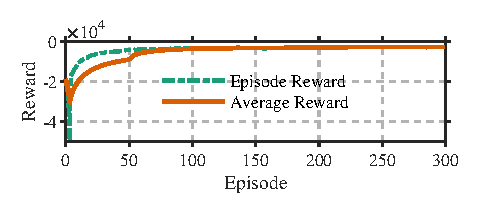
\includegraphics[width=0.8\linewidth]{figs/reward2.eps}
\caption{Training cruve of the PPO-based controller over 300 episodes.}
\label{fig:training_curve}
\end{figure}

\begin{figure}[!t]
\centering
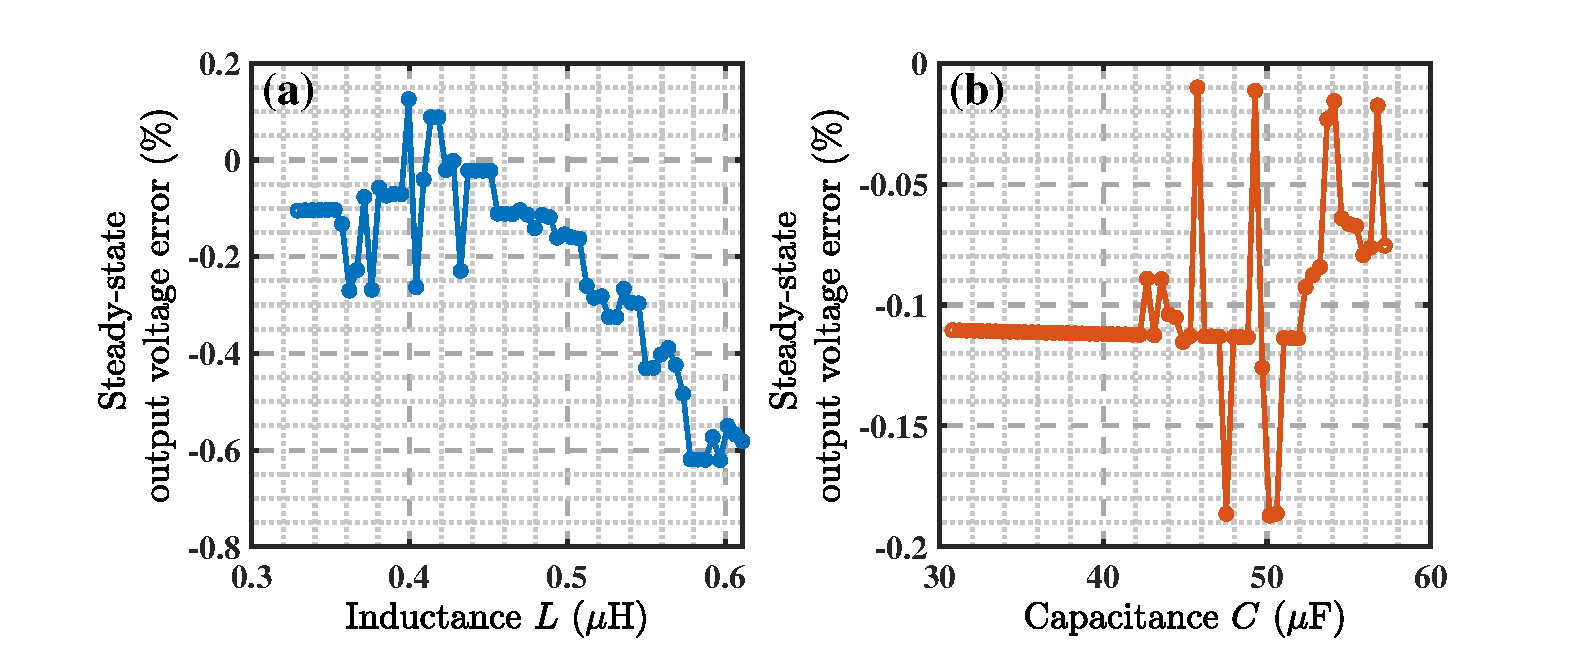
\includegraphics[width=\linewidth]{figs/indcap.eps}
\caption{Steady-state output voltage error under $\pm30\%$ uncertainty in (a) inductance ($0.47\,\mu\text{H}$) and (b) capacitance ($44\,\mu\text{F}$) parameters.}
\label{fig:indcap}
\end{figure}

The results underscore the effectiveness of incorporating action constraints into the reward function. By penalizing excessive control effort, the learned policy achieves improved smoothness and reduced switching noise, thereby enhancing steady-state voltage regulation accuracy.



\begin{figure}[!t]
    \centering
    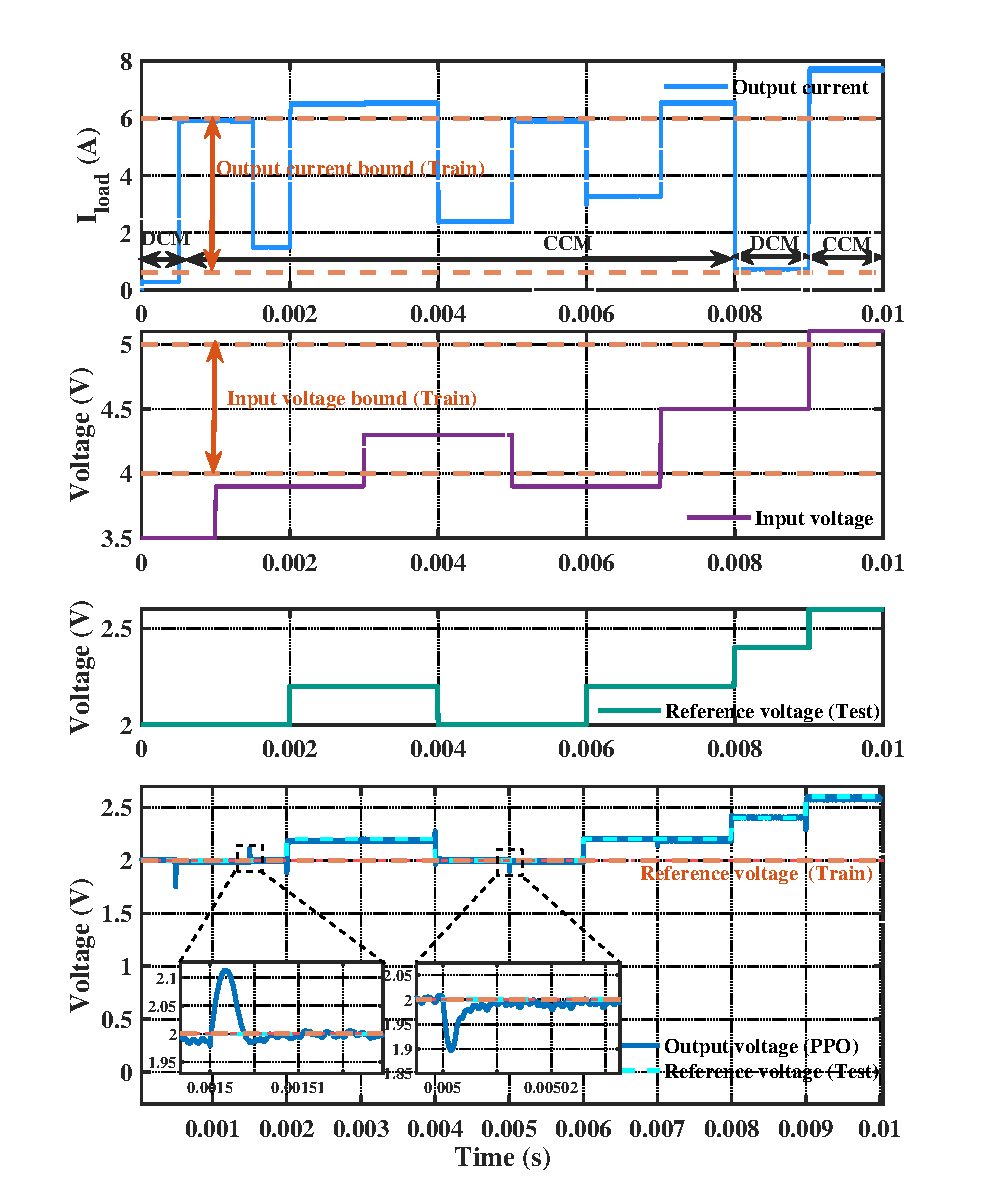
\includegraphics[width=0.95\linewidth]{figs/ccm228.eps} 

    \caption{Results of scenarios where variations in output current, input voltage, and reference voltage occur outside the training range.}
    \label{fig:ccm_dcm}
\end{figure}

\begin{figure}[!t]
\centering
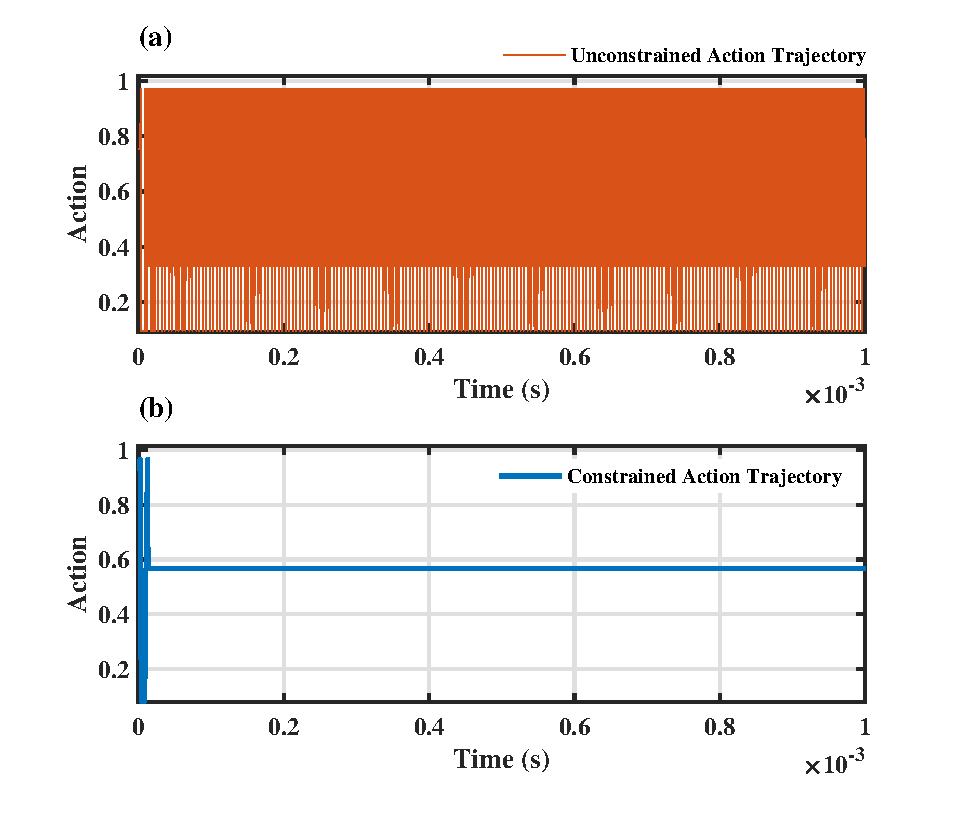
\includegraphics[width=0.48\textwidth]{figs/action_compare3.eps}
\caption{Action trajectories of the PPO-based controller under $V_{\text{in}}=4$\,V, $V_{\text{ref}}=2.2$\,V, and $I_{\text{load}}=3$\,A. (a) Unconstrained action trajectory. (b) Constrained action trajectory.}
\label{fig:action_comparison}
\end{figure}

\begin{figure}[t]
\centering
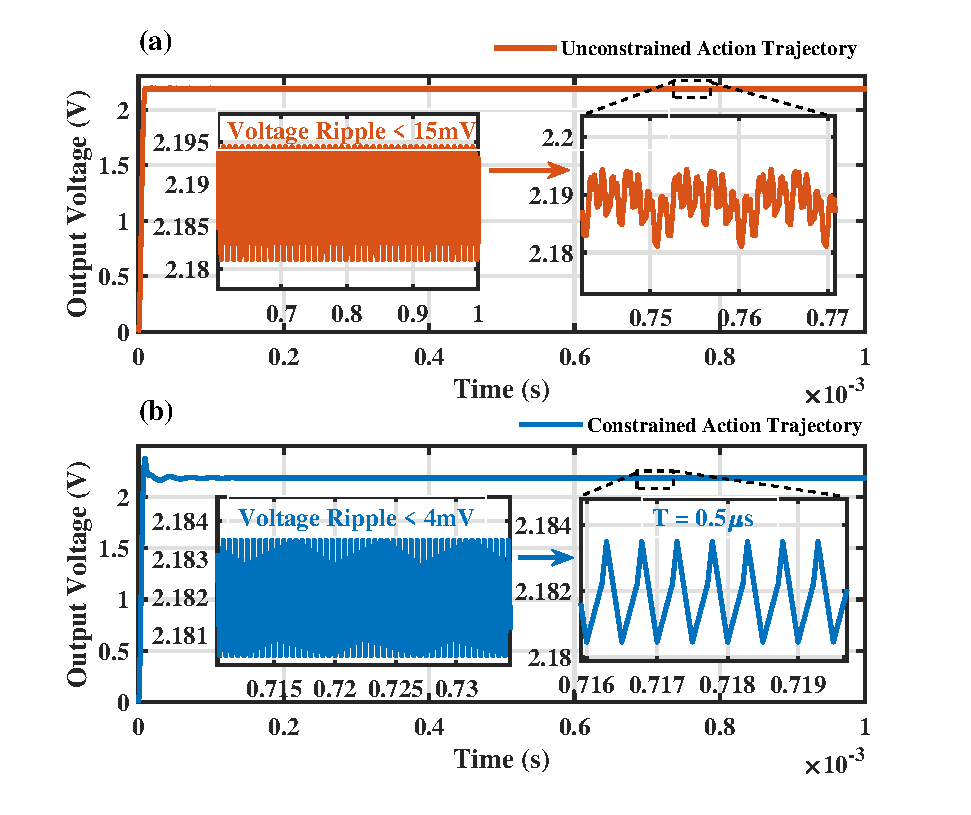
\includegraphics[width=0.48\textwidth]{figs/voltage_action_compar4.eps}
\caption{Output voltage responses under (a) Unconstrained action trajectory. (b) Constrained action trajectory.}
\label{fig:voltage_comparison}
\end{figure}

\section{CONCLUSIONS}

This work proposed a model-free deep reinforcement learning control strategy based on the PPO algorithm for high-frequency DC--DC converter regulation. Trained within a physics-informed simulation environment, the controller achieved fast transient response, minimal overshoot, and accurate steady-state voltage tracking across diverse and dynamic operating conditions. It demonstrated strong robustness under conduction mode transitions (CCM/DCM), parameter uncertainties, and input/load variations. An error-aware reward shaping mechanism was also introduced to suppress oscillations and enforce action smoothness, thereby enhancing voltage stability without compromising dynamic performance. The resulting smooth control behavior effectively reduces switching stress and contributes to improved converter reliability and long-term operational safety.




\bibliographystyle{IEEEtran}
\bibliography{references} 

\end{document}
